\documentclass[12pt]{article}
\usepackage[norsk]{babel} 
\usepackage[utf8]{inputenc} 
\usepackage{times}			% Default times font style
\usepackage[T1]{fontenc} 	% Font encoding
\usepackage{amsmath} 		% Math package


%%Drawing binary trees:
\usepackage{tikz}
\usepackage{verbatim}

\usepackage{hyperref}
\usepackage[letterpaper, margin=1in]{geometry}

\title{}

\begin{document}

\section{Growth of Functions}
\label{sec:1}
Ordering of functions:\\
$2/n$, $37$, $n\log \log n$,
$\sqrt{n}$, $n$, $[n\log n^2$, $n\log n]$, $n\log^2 n$, $n\sqrt{n}$, $n^2$, 
$n^2\log n$, $n^3$, $[\sqrt{2^n}$, $2^n]$

% section 1 (end)

\section{O-notation}
\label{sec:2}
$f$ and $g$ are functions of $n$.

\begin{enumerate}
	\item $O(f*g) = O(f)*O(g)$ is $true$.
	\item Assume $f \equiv C_1\log n$ and $g \equiv C_2\log n$, where $C_1 < C_2$.
	
	Then $O(f) = O(g) = O(\log n)$.
\end{enumerate}
% section 2 (end)

\section{Analysis of Running Time}
\label{sec:3}
There are 8 programs to evaluate, and they give the following number of operations
\begin{enumerate}
	\item $n$
	\item $n/2$
	\item $n^2$
	\item $2n$
	\item $n^3$
	\item $n^2/2$
	\item $n^5/2$
	\item $\log_2 n$
\end{enumerate}
% section 3 (end)
\section{Analysis of Running Time II}
\label{sec:4}

% section 4 (end)
\section{Terminology of Trees and Tree Traversal}
\label{sec:5}
\begin{itemize}
	\item The root of the tree is a.
	\item The leaves are k, l, m.
	\item The height is 5.
	\item When traversing, always go left to right
	\begin{itemize}
	    \item Pre-order: Evaluate node before going to child node(s). Trick: Left dot.
	    
	    \textbf{Result:} a, b, d, g, k, h, c, e, i, f, j, l, m.
	    
	    \item Post-order: Evaluate child nodes before parent node. Trick: Right dot.
	    
	    \textbf{Result:} k, g, h, d, b, i, e, l, m, j, f, c, a.
	    
	    \item In-order: Evaluate left child nodes before parent node. Trick: Middle dot.
	    
	    \textbf{Result:} b, g, k, d, h, a, i, e, c, l, j, m, f.
	    
	    \item Level-order: Evaluate from left to right for each level,
	    starting from the top. 
	    
	    \textbf{Result:} a, b, c, d, e, f, g, h, i, j, k, l, m.
    \end{itemize}
\end{itemize}
% section 5 (end)
\section{Binary Search Tree – Insertion and Deletion}
\label{sec:6}

\begin{figure}[h]
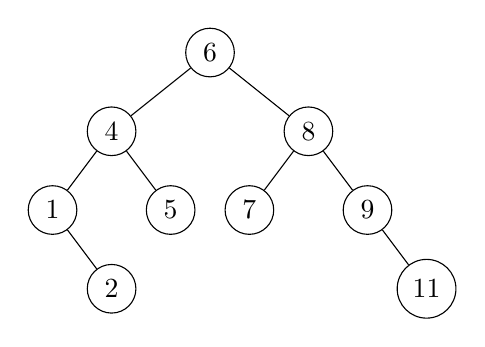
\begin{tikzpicture}[scale=1, every node/.style={circle,draw}]
 \node {6} [level distance=10mm,sibling distance=25mm]
child {node{4} [level distance=10mm ,sibling distance=15mm]
child {node{1}
child[missing]{}
child {node{2}}}
child {node{5}}
}
child {node{8} [level distance=10mm ,sibling distance=15mm]
child {node{7}}
child {node{9}
child[missing]{}
child {node{11}}
}
};
\end{tikzpicture}
\caption{The result of inserting 6, 4, 8, 5, 1, 9, 7, 11, 2 
    into an initially empty binary search-tree.}
\label{fig:tree0}
\end{figure}

\begin{figure}[h]
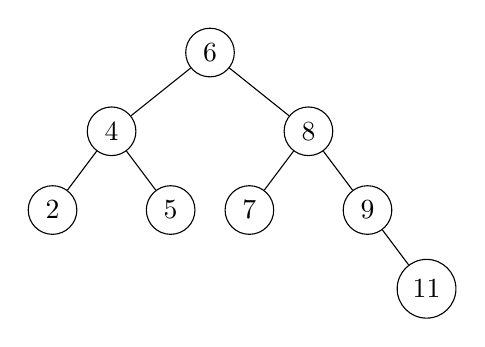
\begin{tikzpicture}[scale=1, every node/.style={circle,draw}]
 \node {6} [level distance=10mm,sibling distance=25mm]
child {node{4} [level distance=10mm ,sibling distance=15mm]
child {node{2}
child[missing]{}
}
child {node{5}}
}
child {node{8} [level distance=10mm ,sibling distance=15mm]
child {node{7}}
child {node{9}
child[missing]{}
child {node{11}}
}
};
\end{tikzpicture}
\caption{The result of deleting 1 from Figure \ref{fig:tree0}.}
\label{fig:tree1}
\end{figure}

\begin{figure}[h]
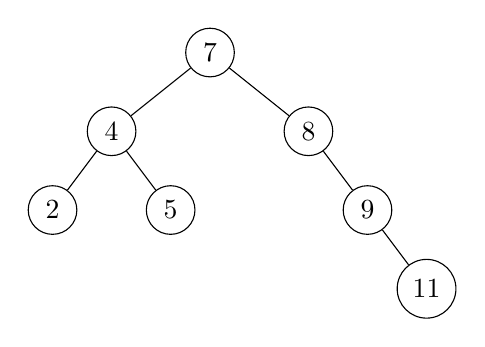
\begin{tikzpicture}[scale=1, every node/.style={circle,draw}]
 \node {7} [level distance=10mm,sibling distance=25mm]
child {node{4} [level distance=10mm ,sibling distance=15mm]
child {node{2}
child[missing]{}
}
child {node{5}}
}
child {node{8} [level distance=10mm ,sibling distance=15mm]
child[missing]{}
child {node{9}
child[missing]{}
child {node{11}}
}
};
\end{tikzpicture}
\caption{The result of deleting 6 from Figure \ref{fig:tree1}.}
\label{fig:tree2}
\end{figure}

% section 6 (end)
\end{document}